\documentclass{beamer}
\usetheme{Boadilla}

\usepackage[czech]{babel}
\usepackage{pdfpages}
\usepackage{graphicx}

\title{Efekt úhlové rychlosti na odraz míčku}
\subtitle{První část experimentu a základ teorie}
\author{Jáchym Löwenhöffer}
\institute{GEVO JM}
\date{\today}

\begin{document}
 
 \begin{frame}
  \titlepage
 \end{frame}

 \begin{frame}{Outline}
  \tableofcontents
 \end{frame}

 \begin{frame}{Nastínění problému}
  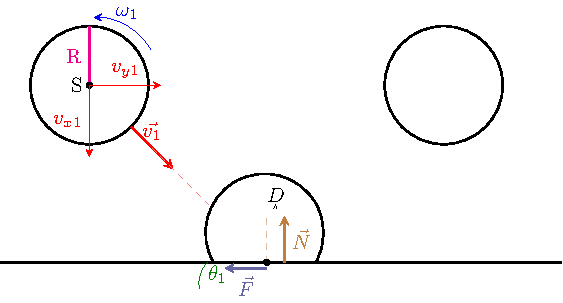
\includegraphics{diagram.pdf}
 \end{frame}

 \section{Teorie} 

\begin{frame}
 \sectionpage
\end{frame}

 \begin{frame}{Teorie}
  Triviální příklady:
  \begin{itemize}
   \item $v_{y1}=0 \Rightarrow $ žádný odraz
   \item $\theta_1\approx0 \Rightarrow v_{x2} > 0$
   \item $\theta_1=90\degree \land \omega_1<0 \Rightarrow v_{x2} < 0 $
   \item $\omega_1=0 \Rightarrow \theta_1=\theta_2 $, Zákon akce a reakce
  \end{itemize}
 \end{frame}

 \begin{frame}{Předpoklady}
 amogus
\end{frame}

\section{Experimenty}
\begin{frame}
 \sectionpage
\end{frame}

 \begin{frame}{Simulace}
 kámo prostě si to doma zkusím ne vole. amogus
\end{frame}
\end{document}

